\documentclass{standalone}
\usepackage{tikz}
\usetikzlibrary{shapes.geometric, arrows}


\definecolor{mycolor}{RGB}{0, 153, 255}
\tikzstyle{process} = [rectangle, rounded corners,
                       minimum width=2cm, minimum height=1cm,
                       text centered, draw=black, fill=mycolor,
                       text=white, line width=0.3mm]

\tikzstyle{arrow} = [thick,->,>=stealth]

\begin{document}
    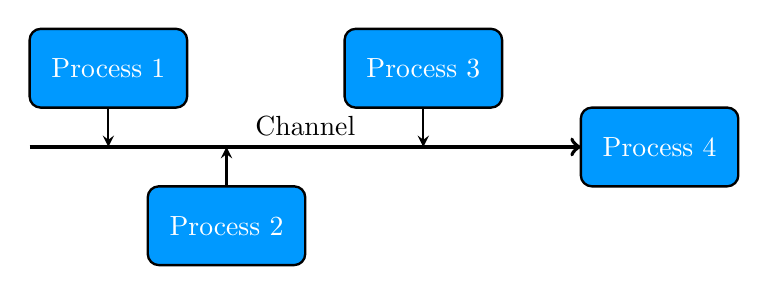
\begin{tikzpicture}[node distance=2cm]
        
        \draw [->, line width=0.5mm] (-1, 0) -- node[anchor=south] {Channel} (6, 0);
        
        \node (Process1) [process, xshift=7cm] {Process 4};
        
        \node (Process2) [process, xshift=0cm, yshift=1cm] {Process 1};
        
        \node (Process3) [process, xshift=1.5cm, yshift=-1cm] {Process 2};
        
        \node (Process4) [process, xshift=4cm, yshift=1cm] {Process 3};
        
        
        \draw [arrow] (0,0.5) -- (0, 0);
        \draw [arrow] (1.5,-0.5) -- (1.5, 0);
        \draw [arrow] (4,0.5) -- (4, 0);
        
        
    
    \end{tikzpicture}
\end{document}
